\documentclass[11pt,letterpaper]{article}

\usepackage[margin=1in]{geometry}
\usepackage[T1]{fontenc}
\usepackage{lmodern}
\usepackage{microtype}
\usepackage{parskip}
\usepackage{enumitem}
\usepackage{booktabs}
\usepackage{longtable}
\usepackage{array}
\usepackage{titlesec}
\usepackage[hidelinks,colorlinks=true,linkcolor=black,urlcolor=black,citecolor=black]{hyperref}
\usepackage{xcolor}
\usepackage{fancyvrb}
\usepackage{fancyhdr}
\usepackage{tikz}
\usetikzlibrary{arrows.meta,positioning,shapes.geometric}

\titleformat{\section}{\Large\bfseries}{\thesection}{1em}{}
\titleformat{\subsection}{\large\bfseries}{\thesubsection}{1em}{}
\titleformat{\subsubsection}{\normalsize\bfseries}{\thesubsubsection}{1em}{}

\pagestyle{fancy}
\fancyhf{}
\fancyhead[L]{\small Theseus Codex --- User Guide}
\fancyhead[R]{\small\thepage}
\renewcommand{\headrulewidth}{0.4pt}

\setlength{\parindent}{0pt}

\newcommand{\mod}[1]{\texttt{#1}}
\newcommand{\pkg}[1]{\textbf{\texttt{#1}}}
\newcommand{\file}[1]{\texttt{#1}}
\newcommand{\page}[1]{\textbf{#1}}
\newcommand{\tab}[1]{\textsl{#1}}

\title{\textbf{The Theseus Codex}\\[4pt]\large A User Guide}
\date{April 2026}
\author{}

\begin{document}

\maketitle
\thispagestyle{empty}

\vspace{2em}

\begin{quote}
\itshape
The Theseus Codex is the web-facing control plane for the firm's epistemic engine. It is where founders upload the raw materials of thinking --- memos, transcripts, essays, live conversations --- and where the engine's output comes back to them as a small number of dashboards they can actually act on.
\end{quote}

\vspace{1em}
\textbf{Live at:} \url{https://mqtheseuswork-qiw6.vercel.app}

\vspace{2em}

\tableofcontents
\newpage

% =======================================================================
\section{What the Codex is (and is not)}
% =======================================================================

The Codex is the screen that founders look at. Everything it shows has been produced by two processes that run \textbf{outside} the browser tab: Noosphere (a Python engine that extracts claims and detects contradictions) and Dialectic (a desktop recorder that transcribes live conversations and auto-uploads the transcripts). The Codex itself does not reason; it renders. Thinking of it this way dissolves most of its apparent complexity --- almost every page is a view over a specific table in the Postgres database.

It is \emph{not}:
\begin{itemize}[leftmargin=*,itemsep=0.2em]
  \item A content management system. You cannot write posts directly in the Codex. Uploads flow in from the outside.
  \item A chat interface. The Codex does not run an LLM conversation.
  \item A publication platform. The \page{Publication} page prepares material for a separate public site; it does not publish anything itself.
  \item A social network. There are no comments, threads, likes.
\end{itemize}

What it \emph{is}: a seven-tab dashboard for the firm's communal brain, with consistent navigation and a one-line explanation at the top of every page.

% =======================================================================
\section{The lifecycle of an idea}
% =======================================================================

Understanding the Codex is easiest as a timeline. A founder has a thought --- in a recorded conversation, in a written memo, in a PDF they read. Here is what happens to it, step by step.

\begin{enumerate}[leftmargin=*,itemsep=0.3em]
  \item \textbf{Capture.} The idea enters the system either through Dialectic (live audio, auto-transcribed to a JSONL file and auto-uploaded) or through the \page{Upload} page (drag-and-drop any text, markdown, or transcript file).

  \item \textbf{Ingest.} Noosphere reads the file and extracts \emph{claims} --- short, declarative, falsifiable statements. Each claim carries an author, a topic, an embedding vector, and a provenance chain linking it back to the source text.

  \item \textbf{Coherence evaluation.} Every new claim is scored against the existing pool on six orthogonal \emph{layers}: natural-language inference, formal argumentation, probabilistic consistency, embedding geometry, information-theoretic compressibility, and an LLM judge. Pairs with a strongly negative aggregated score become \page{Contradictions}; pairs that the layers disagree about become \page{Layer review} items.

  \item \textbf{Synthesis.} Periodically, Noosphere synthesizes firm-level \emph{Conclusions} from groups of mutually supporting claims. Each Conclusion gets one of three tiers: \texttt{open} (tentative, dissent remains), \texttt{founder} (one founder stands behind it), \texttt{firm} (institutional position).

  \item \textbf{Adversarial stress.} For firm-tier Conclusions, the system generates structured objections (\page{Adversarial challenges}) and runs the same six-layer stack against the objection. Challenges that score high and go unaddressed can force a demotion back to \texttt{open}.

  \item \textbf{Calibration.} Any Conclusion that makes a falsifiable prediction enters the \page{Calibration} scoreboard. Resolution dates tick past; outcomes are scored against the predicted probability; Brier / log-loss accumulate by author and domain.

  \item \textbf{Publication (optional).} A firm-tier Conclusion can be pushed into the \page{Publication} queue for internal review. Once approved, it is exported into the firm's public-facing static site with a stable slug, versioned URL, and citation metadata.
\end{enumerate}

Everything in the Codex is a window onto one or more stages of this pipeline.

% =======================================================================
\section{The nav: seven destinations}
% =======================================================================

After consolidation, the top navigation has seven items. Four of them are \emph{group labels} --- clicking one takes you to a default page, and a sub-navigation row appears below the top nav showing the other pages in that group. You never have to hunt for the right URL.

\begin{longtable}{@{}p{0.22\textwidth} p{0.15\textwidth} p{0.55\textwidth}@{}}
\toprule
\textbf{Top nav} & \textbf{Default page} & \textbf{What lives inside} \\
\midrule
\endhead
\page{Dashboard}   & \file{/dashboard}      & Single page. Daily summary of recent uploads, new conclusions, drift events. \\
\page{Upload}      & \file{/upload}         & Single page. Drag-and-drop ingestion form. \\
\page{Conclusions} & \file{/conclusions}    & List of firm claims; click any for a four-tab detail view. \\
\page{Review}      & \file{/contradictions} & Five sub-tabs: \tab{Contradictions}, \tab{Open questions}, \tab{Adversarial}, \tab{Layer review}, \tab{Calibration}. \\
\page{Library}     & \file{/voices}         & Four sub-tabs: \tab{Voices}, \tab{Literature}, \tab{Reading queue}, \tab{Research}. \\
\page{Publication} & \file{/publication}    & Single page. Internal review queue + static-site export. \\
\page{Ops}         & \file{/provenance}     & Seven sub-tabs: \tab{Provenance}, \tab{Eval runs}, \tab{Post-mortem}, \tab{Decay}, \tab{Rigor gate}, \tab{Methods}, \tab{Founders}. \\
\bottomrule
\end{longtable}

Every page, regardless of group, has a consistent banner at the top: page name, one sentence on what it shows, one sentence on when you would use it. That banner is the orientation layer --- nothing below it will make sense if you skipped it.

% =======================================================================
\section{Every page, explained}
% =======================================================================

The per-page guide below walks every destination in the order a new founder would meet them: workspace first, then review, then library, then the operational tabs at the bottom.

\subsection{Workspace}

\subsubsection*{Dashboard \hfill \file{/dashboard}}
\textbf{Shows.} Three blocks side by side: the twelve most recent uploads (with status badges for pending / processing / ingested / failed), the eight newest conclusions (with confidence tier + topic hint), and the six most recent drift events. \\
\textbf{Use it when.} You open the Codex for the day. Nothing here is actionable on its own --- it is a starting point that links deeper.

\subsubsection*{Upload \hfill \file{/upload}}
\textbf{Shows.} A single drag-and-drop form. \\
\textbf{Use it when.} You want to feed a file into the engine manually. Dialectic uploads transcripts automatically; you only use this page for written material or PDFs. \\
\textbf{Supported formats.} \file{.md}, \file{.markdown}, \file{.txt}, \file{.vtt}, \file{.jsonl} are ingested inline (stored as text in Postgres, processed immediately). PDFs, DOCX, and audio files require a binary-storage backend that is not enabled by default on Vercel; they return a clear 413 error with a message pointing at the configuration work still to do.

\subsubsection*{Conclusions \hfill \file{/conclusions}}
\textbf{Shows.} A reverse-chronological list of firm Conclusions, filterable by tier (\texttt{firm} / \texttt{founder} / \texttt{open}) and searchable by topic hint. \\
\textbf{Use it when.} You want to review what the firm believes right now. Each row links to the Conclusion's detail page. \\
\textbf{Temporal replay.} The bar at the top of the list lets you set an \file{asOf} date and see what conclusions would have been consistent with evidence available on or before that date. Replay is a \emph{read projection}, not a literal time machine --- it does not re-run the encoder at historical model versions.

\subsubsection*{Conclusion detail \hfill \file{/conclusions/[id]}}
\textbf{Shows.} Everything about a single Conclusion, across four tabs:
\begin{itemize}[leftmargin=*,itemsep=0.2em]
  \item \tab{Overview}: the Conclusion text, rationale, confidence, supporting principles / evidence chain / dissent counts.
  \item \tab{Provenance}: the extraction chain --- how raw text became this claim, with method + confidence per hop.
  \item \tab{Cascade}: the downstream tree --- what other claims depend on this one, recursively. Useful before retracting.
  \item \tab{Peer review}: founder-cast reviews (endorse / challenge / abstain). You can run a new review here.
\end{itemize}
\textbf{Use it when.} You need to decide whether to trust, cite, or retract a Conclusion.

\subsection{Review: where the firm argues with itself}

\subsubsection*{Contradictions \hfill \file{/contradictions}}
\textbf{Shows.} Claim pairs the coherence engine flagged as incompatible, sorted by severity (0--1). Each row shows the two statements, the severity score, and a JSON breakdown of the six layer verdicts. \\
\textbf{Use it when.} You want the strongest cross-cutting tensions surfaced. Severity above 0.7 is worth a founder look; below 0.5 is usually noise.

\subsubsection*{Open questions \hfill \file{/open-questions}}
\textbf{Shows.} Tensions the system identified but could not resolve automatically. Each item links the two competing claims and summarizes which layers disagreed and why. \\
\textbf{Use it when.} Planning a deliberate-practice session. Open questions are candidates for explicit discussion rather than automated resolution.

\subsubsection*{Adversarial \hfill \file{/adversarial}}
\textbf{Shows.} Structured objections the system generated against firm-tier Conclusions, with coherence scores against the original claim. Challenges are in one of four states: \texttt{pending}, \texttt{addressed} (overridden as answered), \texttt{fallen} (unaddressed, forces conclusion demotion), \texttt{fatal} (human-flagged terminal). \\
\textbf{Use it when.} You want to stress-test institutional positions. The override action on each row is the primary interaction: \texttt{addressed} if the firm has already answered this line of attack in a memo, \texttt{fatal} if it should force the Conclusion to the \texttt{open} tier.

\subsubsection*{Layer review \hfill \file{/q/review}}
\textbf{Shows.} Coherence disputes where the six layers disagreed with each other. The aggregator had to break a tie; your human verdict is solicited to catch cases where it broke wrongly. \\
\textbf{Use it when.} You see a Conclusion whose rationale does not match your intuition, and you want to check whether the layers are unanimous or split.

\subsubsection*{Calibration \hfill \file{/scoreboard}}
\textbf{Shows.} Your firm's prediction track record, broken down by author and domain: Brier score, log-loss, decile-bin calibration. A second section shows firm Conclusions that have calibration-discounted confidence applied. \\
\textbf{Use it when.} You want to know whether you should trust your own firm's probability estimates. Predictions in $[0.45, 0.55]$ are excluded as honest uncertainty --- they are not scored.

\subsection{Library: what the rest of the world has said}

\subsubsection*{Voices \hfill \file{/voices}}
\textbf{Shows.} External thinkers (non-founders) whose claims the system tracks alongside your own: academics, authors, public intellectuals, anyone whose work you have ingested as a source of claims. \\
\textbf{Use it when.} You want to locate the firm's position relative to established thought. Click a voice for their full claim list.

\subsubsection*{Voice detail \hfill \file{/voices/[id]}}
\textbf{Shows.} One voice's claims, grouped by topic, with relative-to-firm stance indicators (agree / disagree / silent). \\
\textbf{Use it when.} Writing about a thinker, or preparing an adversarial session that steelmans a specific perspective.

\subsubsection*{Literature \hfill \file{/literature}}
\textbf{Shows.} External reading material ingested into the evidence pool --- local PDFs, arXiv abstracts, etc. Each item shows license status and whether full text is stored. \\
\textbf{Use it when.} Verifying whether the firm has already ingested a particular paper before recommending it.

\subsubsection*{Reading queue \hfill \file{/reading-queue}}
\textbf{Shows.} Readings the research advisor has suggested, ordered by urgency. Each item is grounded in a specific claim match (you see \emph{why} the advisor thinks this reading is relevant). \\
\textbf{Use it when.} Allocating reading time. Mark items \tab{done} or \tab{skipped} as you work through them; the advisor uses your progress as signal.

\subsubsection*{Research \hfill \file{/research}}
\textbf{Shows.} Topic- and session-level suggestions for the next founder discussion: what to read, what to discuss, which open question to prioritize. \\
\textbf{Use it when.} Planning the agenda for a founder meeting.

\subsection{Publication: the firm's public voice}

\subsubsection*{Publication \hfill \file{/publication}}
\textbf{Shows.} Three panels: the \tab{Queue} (Conclusions enqueued for internal review), the \tab{Reviews} (in-progress and completed), and a \tab{Export} button that produces the JSON bundle consumed by the public static site. \\
\textbf{Use it when.} Moving a firm-tier Conclusion from internal-only to public-facing. Every publish requires an explicit checklist pass (meta-analysis, adversarial engagement, clarity, no leakage, exit conditions declared). The review is the last line of defense against accidental disclosure.

\subsection{Ops: operator and audit surfaces}

These pages support engineers and operators maintaining the firm's epistemic pipeline. Founders touch them less often than the pages above.

\subsubsection*{Provenance \hfill \file{/provenance}}
\textbf{Shows.} Extraction chain for every claim, with extraction method, confidence, and source pointer. Exportable as CSV / JSON. \\
\textbf{Use it when.} Auditing how a specific claim entered the store, or debugging an extractor regression.

\subsubsection*{Eval runs \hfill \file{/eval} and \file{/eval/runs/[runId]}}
\textbf{Shows.} Benchmark runs over the coherence + synthesis pipeline against gold-standard fixtures. The runs list shows macro-F1 and per-domain scores; drilling into a run shows per-case diffs between expected and observed verdicts. \\
\textbf{Use it when.} After a model upgrade, to confirm nothing regressed before rolling out.

\subsubsection*{Post-mortem \hfill \file{/post-mortem}}
\textbf{Shows.} Conclusions that were later retracted, annotated with what the engine originally believed and the evidence that forced the retraction. \\
\textbf{Use it when.} You want a sober read of the firm's failure modes before betting on a tier-2 Conclusion in a high-stakes context.

\subsubsection*{Decay \hfill \file{/decay}}
\textbf{Shows.} Firm Conclusions whose supporting evidence has gone stale: embeddings drifted after an encoder upgrade, claims were superseded, model version no longer matches the fixture. \\
\textbf{Use it when.} You want to prevent bit-rot in the firm's stated positions. The \tab{Revalidate} button re-runs the six-layer stack under the current encoder and updates the Conclusion's decay state.

\subsubsection*{Rigor gate \hfill \file{/rigor-gate} and \file{/rigor-gate/[submissionId]}}
\textbf{Shows.} Publication submissions requiring a rigor-gate check (decorator verification, meta-analysis, adversarial engagement, clarity checklist). Submit new items via the form; click any pending item to see the reviewer checklist. \\
\textbf{Use it when.} Gating anything about to leave the firm (publication, external response, public writing).

\subsubsection*{Methods \hfill \file{/methods}, \file{/methods/candidates}, \file{/methods/[name]/[version]}}
\textbf{Shows.} Registered coherence / synthesis methods the pipeline uses, with their signatures and provenance. Candidates are proposed-but-unreleased variants. Clicking a method version opens its detail page with \tab{Package} (MIP bundle) and \tab{Document} (method card) generation buttons. \\
\textbf{Use it when.} Auditing the firm's methodology for external review, or promoting a candidate method into production.

\subsubsection*{Founders \hfill \file{/founders}}
\textbf{Shows.} Co-founders of the firm with their upload and claim contributions, including topic breakdowns. \\
\textbf{Use it when.} Reviewing who has said what, where the firm's intellectual weight is concentrated.

% =======================================================================
\section{Four workflows, start to finish}
% =======================================================================

Abstract descriptions of pages only go so far. Here are four concrete workflows that exercise the Codex end-to-end.

\subsection{``I want to capture and digest a 90-minute conversation.''}
\begin{enumerate}[leftmargin=*,itemsep=0.2em]
  \item Open Dialectic on your laptop. Start a session. Have the conversation.
  \item Press Stop. Dialectic auto-uploads the transcript to the Codex (assuming \file{DIALECTIC\_CLOUD\_URL} and \file{DIALECTIC\_CLOUD\_API\_KEY} are set).
  \item In the Codex, go to \page{Dashboard}. The new upload appears in the Recent uploads panel. Wait for its status to become \texttt{ingested}.
  \item Go to \page{Conclusions}. Filter by \texttt{topic: <your conversation's topic>} to see newly synthesized firm claims.
  \item Click into any surprising conclusion. Use the \tab{Cascade} tab to see what else depends on it.
  \item Return to \page{Review / Contradictions} to check if anything from the new conversation conflicts with prior positions.
\end{enumerate}

\subsection{``I want to publish the firm's position on X.''}
\begin{enumerate}[leftmargin=*,itemsep=0.2em]
  \item Find the firm-tier Conclusion in \page{Conclusions}.
  \item On its detail page, skim the \tab{Adversarial} tab. Resolve any unaddressed challenges (override as \texttt{addressed} with pointer to memo, or retract the Conclusion if any challenge is \texttt{fatal}).
  \item In \page{Review / Calibration}, check the author's calibration for this domain. If it is weak, consider demoting the Conclusion's public confidence.
  \item Enqueue the Conclusion via \page{Publication / Queue}.
  \item Complete the rigor-gate checklist (meta-analysis, adversarial engagement, clarity, no leakage, exit conditions). Click approve.
  \item Click \tab{Export} to download the public JSON bundle; drop it into \file{theseus-public/content/published.json} and rebuild the static site.
\end{enumerate}

\subsection{``I suspect a conclusion is outdated.''}
\begin{enumerate}[leftmargin=*,itemsep=0.2em]
  \item Go to \page{Ops / Decay}. Scan for conclusions with high decay scores.
  \item Find the conclusion in question; click \tab{Revalidate}. Watch the coherence stack re-run; the decay state updates.
  \item If decay is confirmed, open the conclusion detail, go to \tab{Cascade}, and identify everything downstream.
  \item If major, discuss in the next founder session and retract via \page{Publication} (if public) or directly via the adversarial \texttt{fatal} override (if internal).
\end{enumerate}

\subsection{``I want to know where the firm stands relative to someone else.''}
\begin{enumerate}[leftmargin=*,itemsep=0.2em]
  \item Go to \page{Library / Voices}. Click the voice in question.
  \item Scan their claims list. Each row shows a stance badge: agree / disagree / silent.
  \item Click any \texttt{disagree} row to see which firm Conclusion pushes back, and why.
  \item If gaps show up in the firm's position (many \texttt{silent} on important topics), file a \page{Library / Research} suggestion for next session.
\end{enumerate}

% =======================================================================
\section{Glossary}
% =======================================================================

\begin{description}[leftmargin=*,labelindent=0pt,itemsep=0.3em]
  \item[Claim] A single declarative, falsifiable statement extracted from an upload. The atomic unit of the system. Carries author, topic, embedding, provenance.
  \item[Conclusion] A firm-level synthesized belief derived from multiple supporting claims. Has one of three confidence tiers.
  \item[Confidence tier] \texttt{open} (tentative, dissent present), \texttt{founder} (one founder stands behind it), \texttt{firm} (institutional position).
  \item[Six-layer coherence] Six independent coherence tests applied to every claim pair: NLI, formal argumentation, probabilistic consistency, embedding geometry, information-theoretic compressibility, LLM judge. The aggregator combines them into a single verdict.
  \item[Adversarial challenge] A structured objection the system itself generates against a firm-tier Conclusion. Survives or falls based on coherence against the Conclusion.
  \item[Cascade] The transitive dependency tree rooted at one Conclusion: what other claims and conclusions would need to change if this one were retracted.
  \item[Provenance] The step-by-step extraction chain from raw source text to a structured claim: extractor name, confidence, intermediate transformations.
  \item[Drift event] An observation that a principle or claim's embedding has shifted significantly after recent uploads. Quantitative signal, not a verdict.
  \item[Decay] The opposite arrow: a Conclusion whose supporting evidence has stopped matching the current encoder / world / model. Periodic revalidation is the remedy.
  \item[Rigor gate] A checklist every publication-bound item must pass: methodology declared, adversarial engagement complete, clarity check, no leakage, exit conditions stated.
  \item[Method registry] Versioned, signed record of the extractors and coherence methods the pipeline uses. Enables reproducibility and external audit.
  \item[Calibration-discounted confidence] A Conclusion's stated confidence, adjusted by the author's past Brier performance in the same decile bin. Surfaces only when the feature flag is on.
  \item[Open question] A tension between claims the system raised but could not resolve. Candidate for deliberate-practice discussion.
  \item[Voice] A non-founder thinker whose claims the system tracks for comparison.
  \item[Reading queue] Advisor-suggested readings, ordered by urgency, grounded in claim matches.
  \item[Temporal replay] A read-only projection that shows the Codex as it would have looked given evidence available on a chosen past date. Encoder drift is not undone.
\end{description}

% =======================================================================
\section{Appendix: data flow}
% =======================================================================

\begin{center}
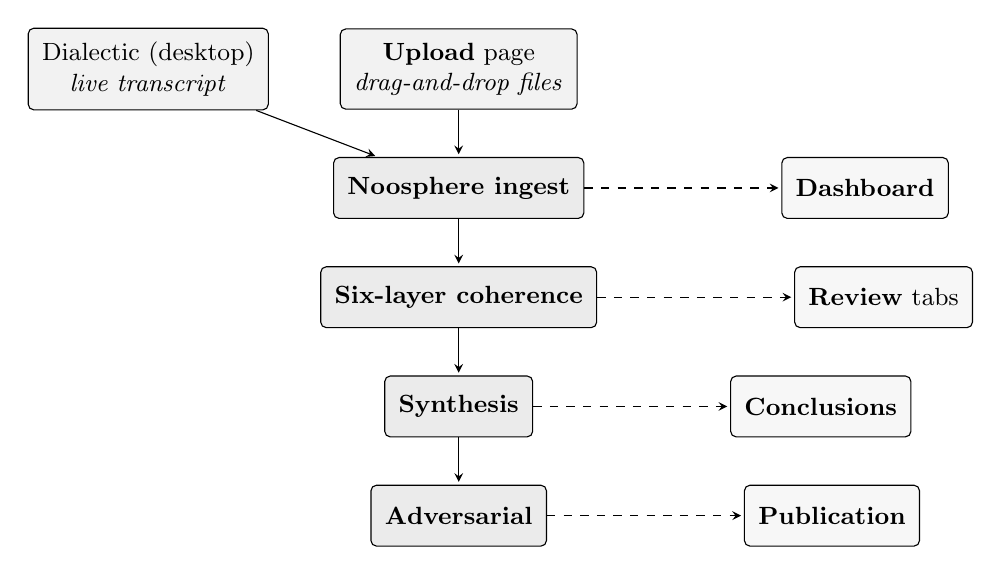
\begin{tikzpicture}[
  node distance=0.6cm and 0.9cm,
  every node/.style={rounded corners=2pt, draw, align=center, font=\small, minimum height=2.2em, inner sep=5pt},
  io/.style={fill=black!5},
  engine/.style={fill=black!8, font=\small\bfseries},
  codex/.style={fill=black!3},
  arr/.style={->, >=stealth, shorten >=1pt}
]
  \node[io] (dialectic) {Dialectic (desktop)\\\emph{live transcript}};
  \node[io, right=of dialectic] (upload) {\page{Upload} page\\\emph{drag-and-drop files}};

  \node[engine, below=of upload] (ingest) {Noosphere ingest};
  \node[engine, below=of ingest] (coh) {Six-layer coherence};
  \node[engine, below=of coh] (synth) {Synthesis};
  \node[engine, below=of synth] (adv) {Adversarial};

  \node[codex, right=2.5cm of ingest] (dash) {\page{Dashboard}};
  \node[codex, right=2.5cm of coh] (rev) {\page{Review} tabs};
  \node[codex, right=2.5cm of synth] (concl) {\page{Conclusions}};
  \node[codex, right=2.5cm of adv] (pub) {\page{Publication}};

  \draw[arr] (dialectic) -- (ingest);
  \draw[arr] (upload) -- (ingest);
  \draw[arr] (ingest) -- (coh);
  \draw[arr] (coh) -- (synth);
  \draw[arr] (synth) -- (adv);

  \draw[arr, dashed] (ingest) -- (dash);
  \draw[arr, dashed] (coh) -- (rev);
  \draw[arr, dashed] (synth) -- (concl);
  \draw[arr, dashed] (adv) -- (pub);
\end{tikzpicture}
\end{center}

\vspace{1em}

Solid arrows are data flowing through the epistemic engine. Dashed arrows are the Codex reading from the database. The Codex never writes into the engine --- it only offers the human-in-the-loop buttons (override, approve, retract) that adjust state, while the engine keeps running in the background.

\end{document}
